\documentclass{beamer}
\usetheme{metropolis}
\usepackage{graphicx}
\usepackage{subfig}
\usepackage{tcolorbox}
\title{Calculus-Based Physics-2: Electricity, Magnetism, and Thermodynamics (PHYS180-02): Unit 1}
\author{Jordan Hanson}
\institute{Whittier College Department of Physics and Astronomy}

\begin{document}
\maketitle

\begin{frame}
\centering
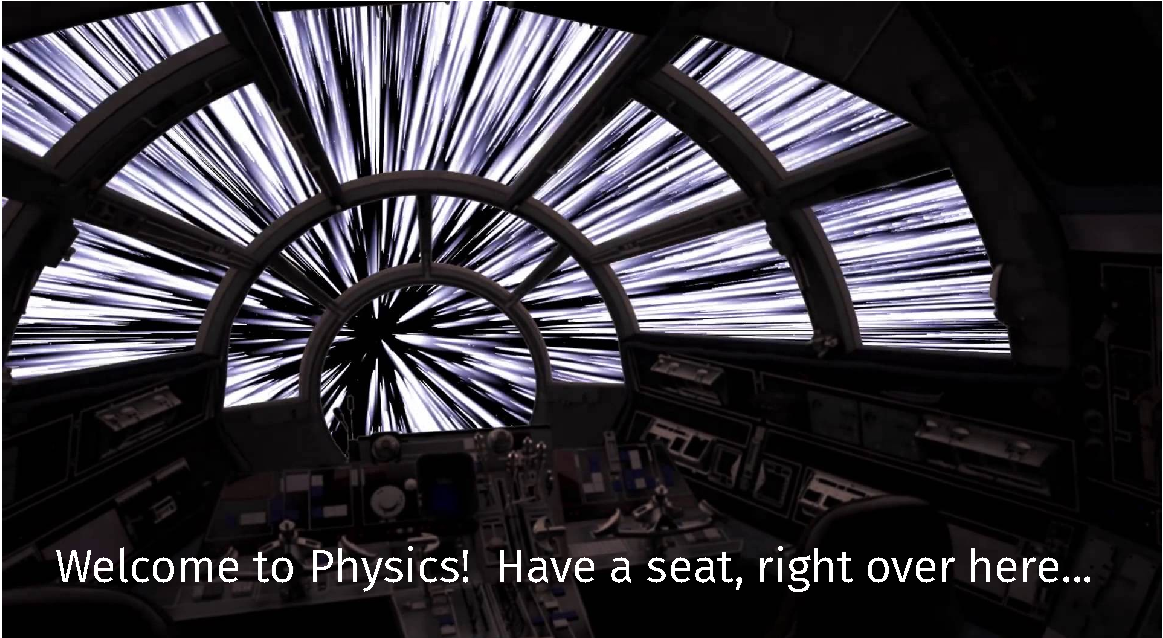
\includegraphics[width=0.95\textwidth]{figures/hyper.pdf}
\end{frame}

\section{Summary}

\begin{frame}{Unit 1 Summary}
\textbf{Reading: Chapters 5-6}
\begin{enumerate}
\item Charge, Conductors and Insulators
\item Coulomb's Law and Electric Fields
\item E-fields of Charge Distributions
\item Gauss's Law
\item Electric Potentials (voltage)
\end{enumerate}
\textbf{Reading for next lecture: all of chapter 5 (electrostatics)} \\ 
\alert{Reading for spring break: chapter 6 (Gauss' Law)} \\
\alert{\textbf{Group presentations:} March 30th} \\
Note that I've had to update the syllabus.
\end{frame}

\section{Charge, Conductors and Insulators}

\begin{frame}{Charge, Conductors and Insulators}
Let's begin this topic in a special way: comparison to \textit{gravity}.  What do electricity and gravity have in common?  The answer lies in a notion we call \textit{charge...}
\end{frame}

\begin{frame}{Charge, Conductors and Insulators}
\centering
\textbf{\alert{Charge: the constant of proportionality between the strength of a \textit{field} and the force a field exerts on an \textit{object}.}} \\
\hrulefill
\small
\begin{columns}[T]
\begin{column}{0.5\textwidth}
\alert{Gravity}
\begin{enumerate}
\item Force: $\vec{F} = G \frac{m M}{r^2} \hat{r}$
\item Parameters: $r$ is absolute distance between two objects with masses $m$ and $M$, and the direction is $\hat{r}$
\item \textit{Charge} of one object: $m$
\item \textit{Field felt by that object}: $\vec{G} = G \frac{M}{r^2} \hat{r}$
\item $\vec{F} = m \vec{G}$
\end{enumerate}
\end{column}
\begin{column}{0.5\textwidth}
\alert{Electricity}
\begin{enumerate}
\item Force: $\vec{F} = k \frac{q Q}{r^2} \hat{r}$
\item Parameters: $r$ is absolute distance between two objects with electric charges $q$ and $Q$, and the direction is $\hat{r}$
\item \textit{Charge} of one object: $q$
\item \textit{Field felt by that object}: $\vec{E} = G \frac{Q}{r^2} \hat{r}$
\item $\vec{F} = q \vec{E}$
\end{enumerate}
\end{column}
\end{columns}
\end{frame}

\begin{frame}{Charge, Conductors and Insulators}
\centering
\textbf{\alert{Charge: the constant of proportionality between the strength of a \textit{field} and the force a field exerts on an \textit{object}.}} \\
\hrulefill \\
\small
In the field paradigm, objects with charges \textit{emanate} fields, causing other objects with charge to experience force. \\
\hrulefill \\
\begin{columns}[T]
\begin{column}{0.5\textwidth}
\alert{Gravity} \\
How many \textit{types of charge}, or how many charges, exist under the force of gravity? \\
\textbf{One.} We call it mass.
\end{column}
\begin{column}{0.5\textwidth}
\alert{Electricity} \\
How many \textit{types of charge}, or how many charges, exist under the force of electricity? \\
\textbf{Two.} We call one positive, and one negative.
\end{column}
\end{columns}
\end{frame}

\begin{frame}{Charge, Conductors and Insulators}
\centering
\textbf{\alert{Charge: the constant of proportionality between the strength of a \textit{field} and the force a field exerts on an \textit{object}.}} \\
\hrulefill \\
\small
In the field paradigm, objects with charges \textit{emanate} fields, causing other objects with charge to experience force. \\
\hrulefill \\
In the field paradigm, gravity has one charge (mass), and electricity has two charges (positive and negative). \\
\hrulefill \\
\textbf{There is one fundamental fact that is puzzling.} What about Newton's 2nd law?  Acceleration is not a field, it is a kinematic function.
\begin{equation}
\vec{F}_{\rm net} = m \vec{a}
\end{equation}
Aparently there are \textit{two kinds of mass}: \textbf{inertial} and \textbf{gravitational}.  
\end{frame}

\begin{frame}{Charge, Conductors and Insulators}
\small
\textit{Equivalence principle:} \\ \hrulefill \\
There are \textit{two kinds of mass}: \textbf{inertial} and \textbf{gravitational}, with \textbf{equal value} for a given object. \\ \vspace{0.5cm}
\url{https://en.wikipedia.org/wiki/Equivalence_principle} \\
\hrulefill \\
There is no similar principle for charge.  If the electric force on a charged object is calculated, that force must still be inserted into \textbf{Newton's 2nd Law} to obtain the acceleration, and the inertial mass must be known.
\end{frame}

\begin{frame}{Charge, Conductors and Insulators}
\small
Charge has other properties, some similar to gravitational mass: \\ \vspace{0.25cm}
\begin{enumerate}
\item Charge is conserved globally (charge cannot be created nor destroyed).  Mass has the same property.
\item Charge is conserved locally (if we pull charge out of the system, charge will flow into the system).
\item Charge is quantized, with an electron (for example) having the fundamental negative unit, and a proton (for example) having the fundamental positive unit.
\item The laws of physics are the same for positive and negative charges.
\item The two kinds of charge emit fields that attract each other; fields emitted by charges of the same type repel such charges.
\end{enumerate}
\end{frame}

\begin{frame}{Charge, Conductors and Insulators}
\textbf{Benjamin Franklin and the Leyden Jar}.  (Good paper topic).
\begin{figure}
\centering
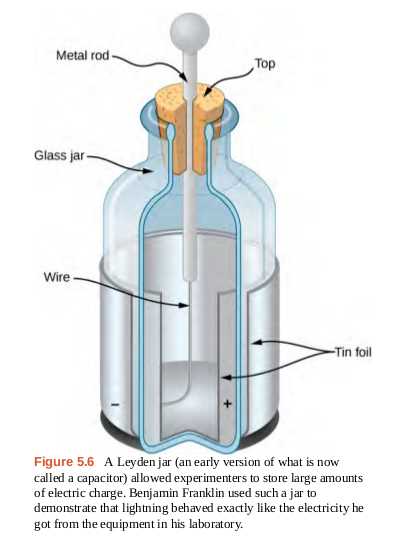
\includegraphics[width=0.3\textwidth]{figures/leyden.png}
\caption{\label{fig:leyden} A Leyden jar was an early version of a capacitor.  Benjamin Franklin guessed that one type of charge moves and another remains stationary, explaining several behaviors of charged objects.}
\end{figure}
\end{frame}

\begin{frame}{Charge, Conductors and Insulators}
The rest of the properties of charge are connected to the development of the structure of the atom, and we will return to this topic at the end of the semeter.
\begin{figure}
\centering
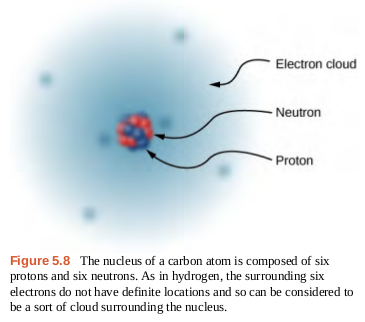
\includegraphics[width=0.5\textwidth]{figures/atom.png}
\caption{\label{fig:atom} A sketch of our current atomic paradigm.}
\end{figure}
\end{frame}

\begin{frame}{Charge, Conductors and Insulators}
Suppose an ion is composed of six protons, eight neutrons, and five electrons.  What is the net charge?
\begin{itemize}
\item A: +1
\item B: 0
\item C: -1
\item D: -2
\end{itemize}
\end{frame}

\begin{frame}{Charge, Conductors and Insulators}
A rod with a positive charge is held next to a \textit{conductor} (an object were charge can move around freely).  Which of the following is true?
\begin{itemize}
\item A: The charges in the conductor all remain in place because charge is conserved.
\item B: The negative charges in the conductor move toward the positive charges in the rod.
\item C: The positive charges remain in place but the negative charges move away from the rod.
\item D: The positive charges move toward the rod and the negative charges remain in place.
\end{itemize}
\end{frame}

\section{Coulomb’s Law and Electric Fields}

\begin{frame}{Coulomb’s Law and Electric Fields}
\textbf{Coulomb's Law} describes the force between charges. \\ \vspace{0.5cm}
\begin{tcolorbox}[colback=white,colframe=red!40!blue,title=Coulomb's Law]
\alert{The electric force, or \textbf{Coulomb force}, between two electrically charged systems with charges $q_{\rm 1}$ and $q_{\rm 2}$ separated by a distance $r$ is
\begin{equation}
\vec{F}_{\rm C} = \frac{1}{4\pi\epsilon_{\rm 0}} \frac{q_{\rm 1} q_{\rm 2}}{r^2} \hat{r} \label{eq:C}
\end{equation}
In Eq. \ref{eq:C}, $\hat{r} = \vec{r}/|\vec{r}|$, and $\epsilon_{\rm 0} = 8.85418782\times 10^{-12} N^{-1} m^{-2} C^2$, called the \textit{perimittivity of free space.}}
\end{tcolorbox}
\end{frame}

\begin{frame}{Coulomb’s Law and Electric Fields}
\begin{tcolorbox}[colback=white,colframe=red!40!blue,title=Coulomb Field]
\alert{The electric field corresponding to Eq. \ref{eq:C}, experienced by a charge $q$ and generated by a charge $Q$ is 
\begin{equation}
\vec{E}_{\rm C} = \frac{1}{4\pi\epsilon_{\rm 0}} \frac{Q}{r^2} \hat{r} \label{eq:Cf}
\end{equation}
In Eq. \ref{eq:Cf}, $r$ remains the separation between $q$ and $Q$.}
\end{tcolorbox}
Thus we have: $\vec{F}_{\rm C} = q \vec{E}_{\rm C}$. \\ \vspace{0.5cm}
The SI Unit of charge is the Coulomb, which is equal to the amount of charge in a "current" of 1 amp for 1 second (more on this later).  \textbf{The charge of an electron is $1.6\times 10^{-19}$ Coulombs, or C.}
\end{frame}

\begin{frame}{Coulomb’s Law and Electric Fields}
Suppose a charge $+q$ experiences the Coulomb field of another charge of $-2q$, separated by a distance $r$.  Which of the following is true?
\begin{itemize}
\item A: The charge $+q$ accelerates towards the other charge, and the charge $-2q$ remains stationary, because opposite charges attract.
\item B: The charge $-2q$ accelerates towards the other charge, and the charge $+q$ remains stationary, because opposite charges attract.
\item C: No charges move; the force on one is equal to the force on the other.
\item D: The charges accelerate towards each other.
\end{itemize}
\end{frame}

\begin{frame}{Coulomb’s Law and Electric Fields}
The answer to the previous problem involves Newton's Third Law.  (\textit{Why did only the negative charges move})?
\begin{figure}
\centering
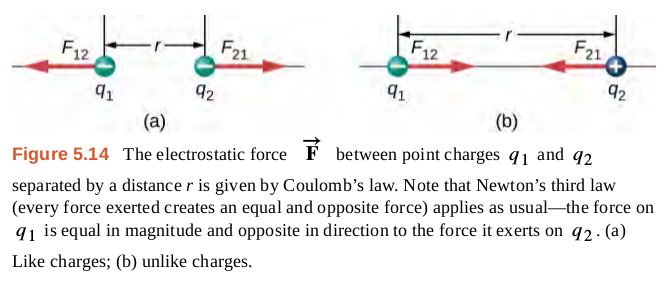
\includegraphics[width=0.9\textwidth]{figures/third.png}
\caption{\label{fig:third} Newton's Third Law still applies.}
\end{figure}
\end{frame}

\begin{frame}{Coulomb’s Law and Electric Fields}
Suppose a charge $+q$ experiences the Coulomb fields of two other charges of $-2q$, each located a distance $r$ from $+q$.  The charges are all colinear (on the same line).  Which of the following is true?
\begin{itemize}
\item A: The charge $+q$ accelerates towards one of the other charge, because opposite charges attract.
\item B: The charges $-2q$ accelerate towards the charge $+q$.
\item C: The charges $-2q$ accelerate towards the charge $+q$, but eventually repel each other back in the other direction.
\item D: The charges $-2q$ repel each other from the start.
\end{itemize}
\end{frame}

\begin{frame}{Coulomb’s Law and Electric Fields}
\small
The Coulomb force equation gives a vector, and so does the corresponding electric field.  Like a gravitational field, this effect has a vector at each point in space, so we refer to the Coulomb force and the Coulomb field as \textit{vector fields}. \\ \vspace{0.5cm}
\textbf{Vector field}: An assignment of a vector to each point in a subset of space.
\end{frame}

\begin{frame}{Coulomb’s Law and Electric Fields}
\small
\begin{columns}[T]
\begin{column}{0.5\textwidth}
Which of the following is true of vectors $\vec{v}_{\rm i}$ in the lower left-hand corner of the figure at right?
\begin{itemize}
\item A: They are probably $\vec{v}_{\rm i} = -\hat{i}-\hat{j}$
\item B: They are probably $\vec{v}_{\rm i} = \hat{i}+\hat{j}$
\item C: They are probably $\vec{v}_{\rm i} = -\hat{i}+\hat{j}$
\item D: They are probably $\vec{v}_{\rm i} = \hat{i}-\hat{j}$
\end{itemize}
\end{column}
\begin{column}{0.5\textwidth}
\begin{figure}
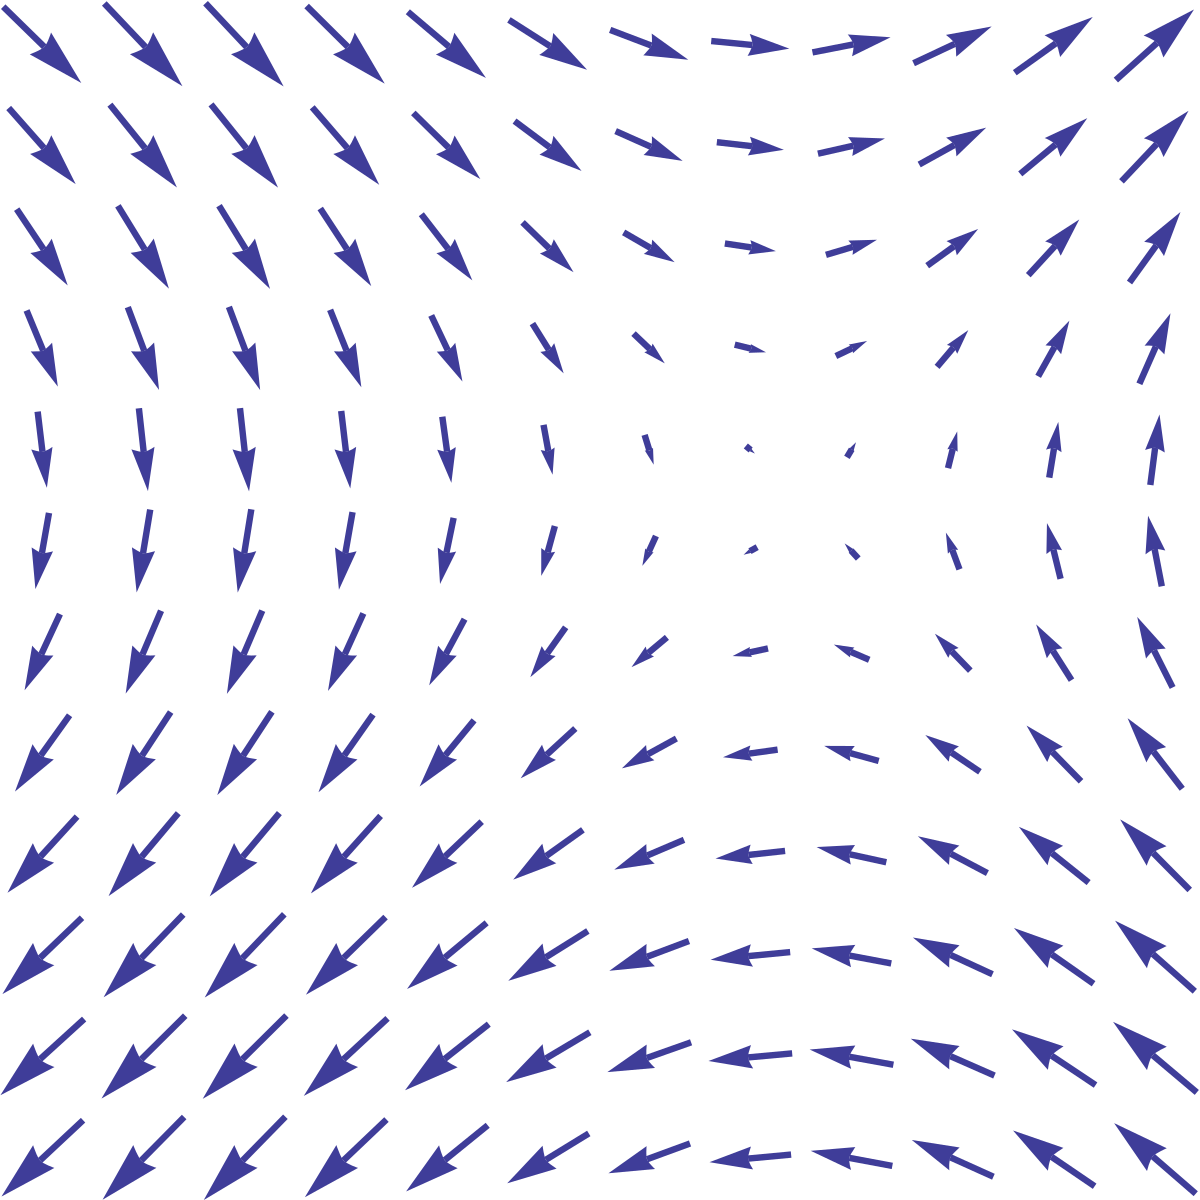
\includegraphics[width=\textwidth]{figures/vectorField.png}
\caption{\label{fig:field} A vector field of vectors $\vec{v}_{\rm i}$.  Let $\hat{j}$ represent up, and $\hat{i}$ represent right.}
\end{figure}
\end{column}
\end{columns}
\end{frame}

\begin{frame}{Coulomb’s Law and Electric Fields}
\small
\begin{columns}[T]
\begin{column}{0.5\textwidth}
Which of the following is true of vectors $\vec{v}_{\rm i}$ in the upper left-hand corner of the figure at right?
\begin{itemize}
\item A: They are probably $\vec{v}_{\rm i} = -\hat{i}-\hat{j}$
\item B: They are probably $\vec{v}_{\rm i} = \hat{i}+\hat{j}$
\item C: They are probably $\vec{v}_{\rm i} = -\hat{i}+\hat{j}$
\item D: They are probably $\vec{v}_{\rm i} = \hat{i}-\hat{j}$
\end{itemize}
\end{column}
\begin{column}{0.5\textwidth}
\begin{figure}
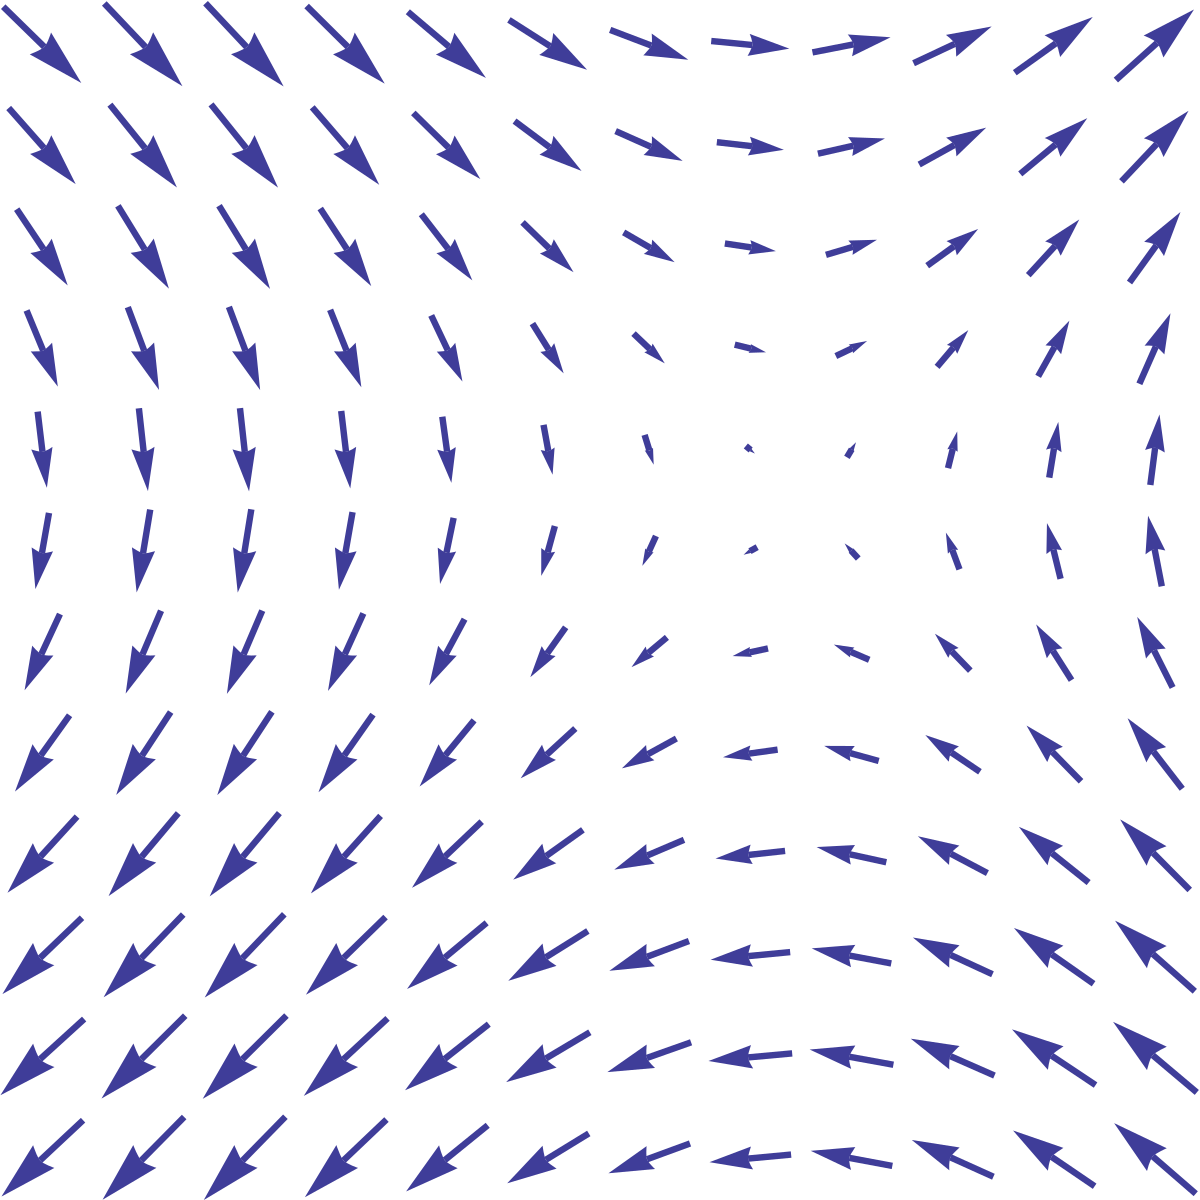
\includegraphics[width=\textwidth]{figures/vectorField.png}
\caption{\label{fig:field2} A vector field of vectors $\vec{v}_{\rm i}$.  Let $\hat{j}$ represent up, and $\hat{i}$ represent right.}
\end{figure}
\end{column}
\end{columns}
\end{frame}

\begin{frame}{Coulomb’s Law and Electric Fields}
\small
\begin{columns}[T]
\begin{column}{0.5\textwidth}
\textbf{Group board exercise}: What is the angle of the net electric field for the \textit{test charge} at the point (1,1) in Fig. \ref{fig:netfield1}? \\ \vspace{0.5cm}
\textbf{Group board exercise}: What is the magnitude of the net electric field for the \textit{test charge} at the point (1,1) in Fig. \ref{fig:netfield1}, if the distances have units of nanometers, and $q$ is the charge of an electron, $1.6\times 10^{-19}$ C? (Let $\frac{1}{4\pi\epsilon_{\rm 0}} = 9\times 10^{9}$ N m$^2$ C$^{-2}$).\\ \vspace{0.5cm}
\end{column}
\begin{column}{0.5\textwidth}
\begin{figure}
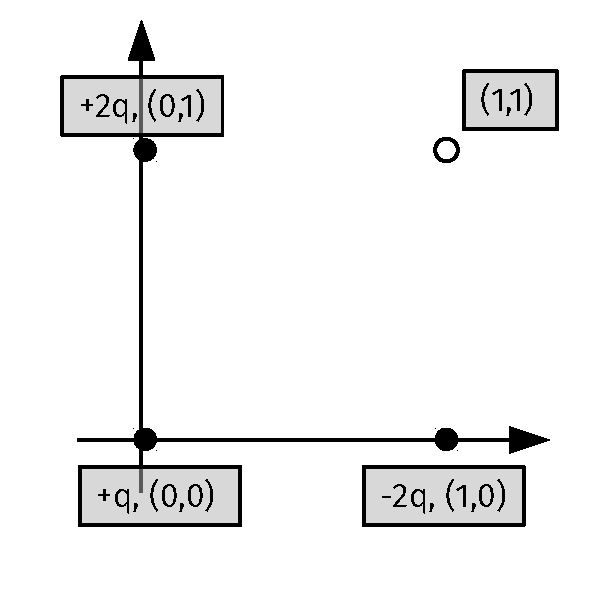
\includegraphics[width=\textwidth]{figures/NetField1.pdf}
\caption{\label{fig:netfield1} Three charges create a field for a hypothetical \textit{test charge}.}
\end{figure}
\end{column}
\end{columns}
\end{frame}

\begin{frame}{Coulomb’s Law and Electric Fields}
\small
\begin{columns}[T]
\begin{column}{0.5\textwidth}
What is the angle of the E-field at point (1,1) in Fig. \ref{fig:netfield2} at right?
\begin{itemize}
\item A: 0 deg
\item B: 45 deg
\item C: 90 deg
\item D: 135 deg
\end{itemize}
What is the fastest way to solve this problem?
\begin{itemize}
\item A: Blind luck
\item B: Do the algebra
\item C: Symmetry
\item D: Numerical estimation
\end{itemize}
\end{column}
\begin{column}{0.5\textwidth}
\begin{figure}
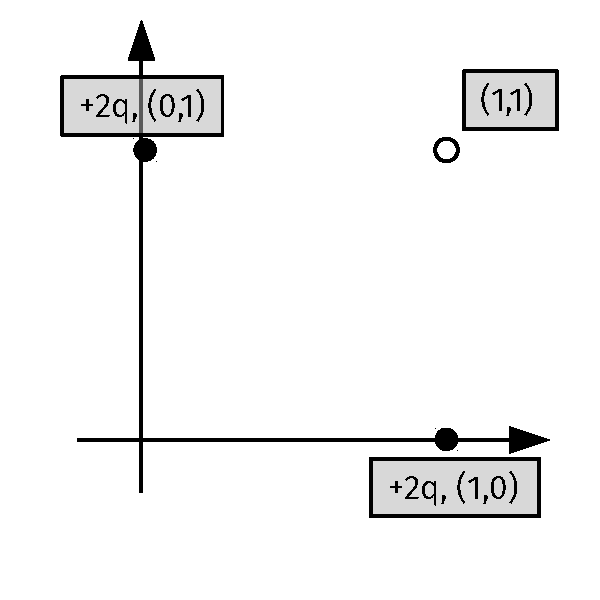
\includegraphics[width=\textwidth]{figures/NetField2.pdf}
\caption{\label{fig:netfield2} Two charges create a field for a hypothetical \textit{test charge}.}
\end{figure}
\end{column}
\end{columns}
\end{frame}

\begin{frame}{Coulomb’s Law and Electric Fields}
\small
\begin{columns}[T]
\begin{column}{0.5\textwidth}
What is the angle of the E-field at point (1,1) in Fig. \ref{fig:netfield3} at right?
\begin{itemize}
\item A: About 0 deg
\item B: About 25 deg
\item C: About 45 deg
\item D: About 60 deg
\end{itemize}
\end{column}
\begin{column}{0.5\textwidth}
\begin{figure}
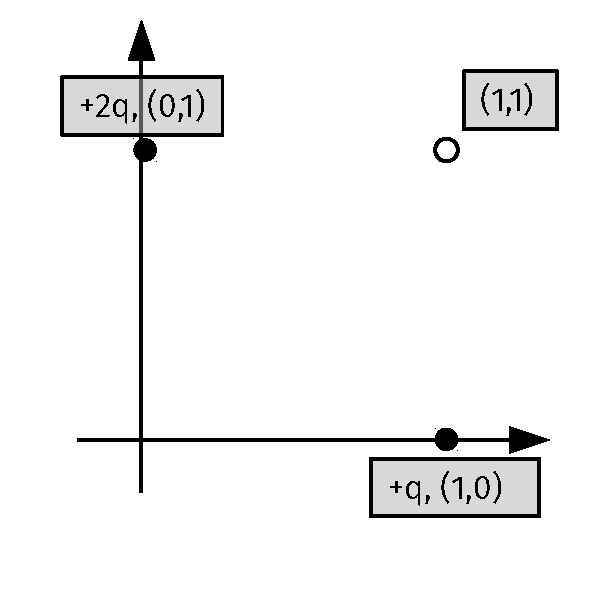
\includegraphics[width=\textwidth]{figures/NetField3.pdf}
\caption{\label{fig:netfield3} Two charges create a field for a hypothetical \textit{test charge}.}
\end{figure}
\end{column}
\end{columns}
\end{frame}

\begin{frame}{Coulomb’s Law and Electric Fields}
The forces of $N$ fixed charges on a test charge $Q$ create a net force, where the individual forces simply add like vectors.  This is known as the \textbf{superposition principle}.
\begin{align}
\vec{F}_{\rm C,Net} &= \frac{1}{4\pi\epsilon_{\rm 0}} Q \sum_{i = 1}^N \frac{q_i}{r_i^2}\hat{r}_i = Q \vec{E}_{\rm C,Net} \\
\vec{E}_{\rm C,Net} &= \frac{1}{4\pi\epsilon_{\rm 0}} \sum_{i = 1}^N \frac{q_i}{r_i^2}\hat{r}_i
\end{align}
\end{frame}

\begin{frame}{Coulomb’s Law and Electric Fields}
For the expressions of fields built from the superposition principle, let's adopt a notation:
\begin{equation}
\vec{E}_{\rm C,Net}(P) = \frac{1}{4\pi\epsilon_{\rm 0}} \sum_{i = 1}^N \frac{q_i}{r_i^2}\hat{r}_i \label{eq:P}
\end{equation}
Equation \ref{eq:P} represents the field at a \textit{position} $P = P(x,y,z)$, relative to the positions $\vec{r}_i$ of the source charges.
\end{frame}

\begin{frame}{Coulomb’s Law and Electric Fields}
\small
\begin{columns}[T]
\begin{column}{0.5\textwidth}
\textbf{Table exercise:} Calculate $\vec{E}_{\rm C,Net}(P)$, if $P = (1,1)$. \\ \vspace{0.5cm}
\textbf{Table exercise:} Calculate $\vec{E}_{\rm C,Net}(P)$, if $P = (-1,-1)$. \\ \vspace{0.5cm}
\textbf{Group discussion:} What does it mean if $P = (1,0)$? \\ \vspace{0.5cm}
\end{column}
\begin{column}{0.5\textwidth}
\begin{figure}
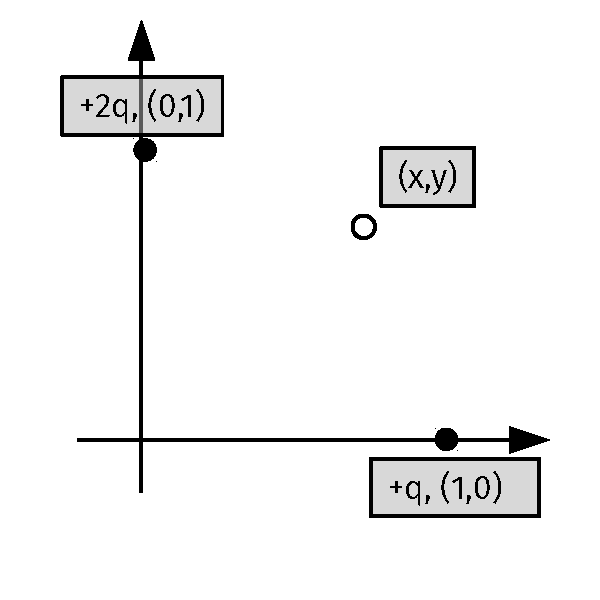
\includegraphics[width=\textwidth]{figures/NetField4.pdf}
\caption{\label{fig:netfield4} Two charges create a field for a hypothetical \textit{test charge}.}
\end{figure}
\end{column}
\end{columns}
\end{frame}

\begin{frame}{Coulomb’s Law and Electric Fields}
Notice in the prior examples of \textit{fixed} charges, we need an \textit{explanation} for why the fixed charges remain fixed, even though they are obviously subject to Coulomb forces. \\ \vspace{0.5cm}
\textbf{Insulator}: A material in which there are no free charges available to conduct electricity.  Charges may be fixed in position within an insulator. \\
\textbf{Conductor}: A material in which there are free charges available to conduct electricity.  Charges may not be fixed in position within a conductor. \\
\textbf{Semi-conductor}: A material in which there are free charges available to conduct electricity if certain requirements are met.
\end{frame}

\begin{frame}{Coulomb’s Law and Electric Fields}
\small
\begin{columns}[T]
\begin{column}{0.5\textwidth}
The following problem is an example of solving for a field analytically, and \textit{testing various limits}.  Upon taking limits results are often simple and intuitive. \\ \vspace{0.5cm}
Two charges $+q$ are on the fixed in an insulator on the x-axis.  Solve for the E-field at $P = (0,0,z)$. \\ \vspace{0.5cm}
Show that the general solution is
\begin{equation}
\vec{E}(z) = \frac{1}{4\pi\epsilon_0} \frac{2qz}{\left(z^2+\left(\frac{d}{2}\right)^2\right)^{3/2}} \hat{k}
\end{equation}
\end{column}
\begin{column}{0.5\textwidth}
\begin{figure}
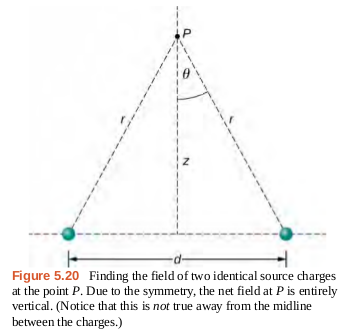
\includegraphics[width=\textwidth]{figures/twoChargesZ.png}
\caption{\label{fig:twoChargesZ} Solve for the E-field as a function of $z$, $d$, and $q$.}
\end{figure}
\end{column}
\end{columns}
\end{frame}

\begin{frame}{Coulomb’s Law and Electric Fields}
\small
\begin{columns}[T]
\begin{column}{0.5\textwidth}
Show that the general solution is
\begin{equation}
\vec{E}(z) = \frac{1}{4\pi\epsilon_0} \frac{2qz}{\left(z^2+\left(\frac{d}{2}\right)^2\right)^{3/2}} \hat{k}
\end{equation}
\textit{Take the following two limits:} \\ 1) $z \gg d$ and 2) $z=0$.  What are the results? \\ \vspace{0.5cm}
Keep these results in mind, because we are about to start drawing \textbf{vector fields,} in order to visualize the algebra.
\end{column}
\begin{column}{0.5\textwidth}
\begin{figure}
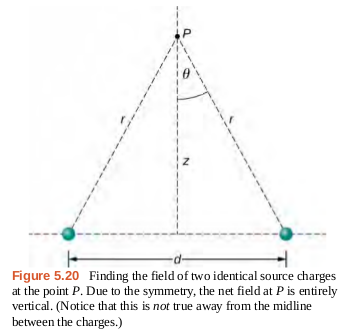
\includegraphics[width=\textwidth]{figures/twoChargesZ.png}
\caption{\label{fig:twoChargesZ2} Solve for the E-field as a function of $z$, $d$, and $q$.}
\end{figure}
\end{column}
\end{columns}
\end{frame}

\begin{frame}{Coulomb’s Law and Electric Fields}
\textbf{PhET Simulation of E-fields from Charges}: \\ \vspace{0.5cm}
\url{https://phet.colorado.edu/en/simulation/charges-and-fields}
\begin{enumerate}
\item Create the situation in the prior problem, in Fig. \ref{fig:twoChargesZ2}.
\item Use the yellow sensor object to determine the local direction of the E-field at various points along the z-axis.
\begin{itemize}
\item Do the results match the limit $z\gg d$?
\item Do the results match the limit $z = 0$, halfway between the charges?
\item Where is the field maximal?
\end{itemize}
\item Make sure you can see above and below the charges, and repeat steps 1 and 2 for negative z-values.  What do you find?
\end{enumerate}
\end{frame}

\begin{frame}{Coulomb’s Law and Electric Fields}
\small
\textbf{PhET Simulation of E-fields from Charges}: \\ \vspace{0.5cm}
Build E-fields with the following properties, by adding single charges.  Let the \textit{z-axis be upwards}, and let the \textit{x-axis be to the right.}
\begin{enumerate}
\item Build an electric field that has \textbf{reflection symmetry} across the z-axis, with at least five charges.
\item Build an electric field that has \textit{radial symmetry} about the origin, with at least six charges.
\item Build an electric field that would be the same if I rotated the picture by 90 degrees (\textbf{4-fold symmetry}) with at least four charges, some negative and some positive.
\item Build an electric field that would be the same if I rotated the picture by 45 degrees (\textbf{8-fold symmetry}) with at least eight charges, some negative and some positive.
\end{enumerate}
\end{frame}

\begin{frame}{Coulomb’s Law and Electric Fields}
\small
\textbf{PhET Simulation of E-fields from Charges}: \\ \vspace{0.5cm}
\alert{The lesson is that the E-field has the \textit{symmetry properties} of the \textit{charge distribution}}.
\end{frame}

\begin{frame}{Coulomb’s Law and Electric Fields}
When we connect the vectors in a vector field, the results are figures like Fig. \ref{fig:lines}.  Fields by convention originate from positive charges and terminate on negative ones.
\begin{figure}
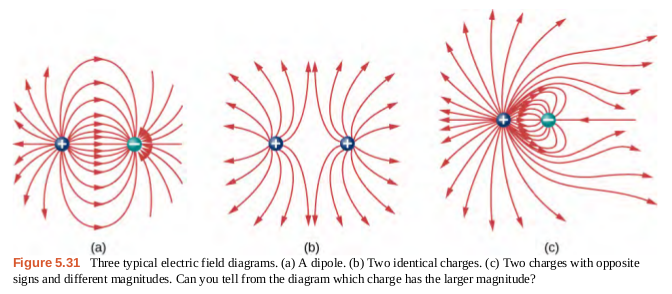
\includegraphics[width=0.8\textwidth]{figures/lines.png}
\caption{\label{fig:lines} Field-line diagrams.  The density of lines indicates electric field strength.}
\end{figure}
\end{frame}

\section{E-Fields of Charge Distributions}

\begin{frame}{E-Fields of Charge Distributions}
Welcome to calculus! Let $k = 1/(4\pi\epsilon_0)$.
\begin{align}
\vec{E}(P) &= k \sum_{i = 1}^N \left(\frac{q_i}{r_i^2}\right) \hat{r} \label{eq:point} \\
\vec{E}(P) &= k \int_{line} \left(\frac{\lambda dl}{r^2}\right) \hat{r} \label{eq:line} \\
\vec{E}(P) &= k \int_{surface} \left(\frac{\sigma dA}{r^2}\right) \hat{r} \label{eq:surface} \\
\vec{E}(P) &= k \int_{volume} \left(\frac{\rho dV}{r^2}\right) \hat{r} \label{eq:volume}
\end{align}
The functions $\lambda$, $\sigma$, and $\rho$ are just charge densities.  They decribe where charge is, and how much there is.  
\end{frame}

\begin{frame}{E-Fields of Charge Distributions}
\begin{figure}
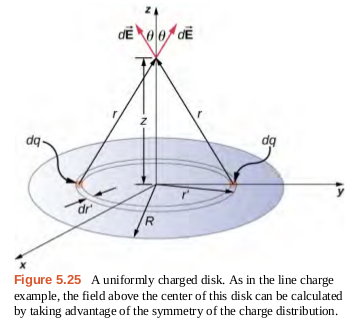
\includegraphics[width=0.45\textwidth]{figures/disk.png}
\caption{\label{fig:disk} We are going to work this example together, and other examples will be left to homework.}
\end{figure}
\textbf{Observe on board.}
\end{frame}

\begin{frame}{E-Fields of Charge Distributions}
\begin{figure}
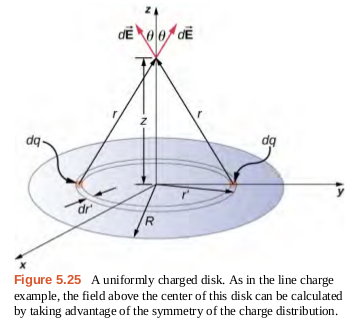
\includegraphics[width=0.4\textwidth]{figures/disk.png}
\caption{\label{fig:disk2} We are going to work this example together, and other examples will be left to homework.}
\end{figure}
Result:
\begin{equation}
\boxed{
\vec{E} = k\left(2\pi\sigma - \frac{2\pi\sigma z}{\sqrt{R^2 + z^2}} \right)\hat{k}}
\end{equation}
\end{frame}

\begin{frame}{E-Fields of Charge Distributions}
\begin{equation}
\boxed{
\vec{E} = k\left(2\pi\sigma - \frac{2\pi\sigma z}{\sqrt{R^2 + z^2}} \right)\hat{k}} \label{eq:disk}
\end{equation}
Which of the following not true of Eq. \ref{eq:disk}?
\begin{itemize}
\item A: Taking the limit $R \rightarrow \infty$ yields a constant field.
\item B: Taking the limit $z \rightarrow 0$ yields a constant field.
\item C: The charge distribution has radial symmetry, so the field cannot have horizontal components.
\item D: Taking the value $z = R$ represents a minimum in the field strength.
\end{itemize}
\end{frame}

\begin{frame}{E-Fields of Charge Distributions}
\begin{equation}
\boxed{
\vec{E} = k\left(2\pi\sigma - \frac{2\pi\sigma z}{\sqrt{R^2 + z^2}} \right)\hat{k}} \label{eq:disk2}
\end{equation}
What happens to Eq. \ref{eq:disk2}, in the limit that $R \rightarrow \infty$?
\begin{itemize}
\item A: The field decreases to zero.
\item B: The field is constant.
\item C: The field grows increasingly positive.
\item D: The field grows increasingly negative.
\end{itemize}
\end{frame}

\begin{frame}{E-Fields of Charge Distributions}
In the limit that $R \rightarrow \infty$,
\begin{equation}
\vec{E} = 2\pi\sigma k \hat{k} = \frac{\sigma}{2\epsilon_0} \hat{k} \label{eq:disk3}
\end{equation}
Equation for the electric field of a uniform infinite disk.
\end{frame}

\begin{frame}{E-Fields of Charge Distributions}
Imagine two infinite disks with equal uniform charge distributions, some distance apart.  One has positive charge, the other negative charge.  What is the E-field between them?
\begin{itemize}
\item A: 0
\item B: $\frac{\sigma}{2\epsilon_0}$
\item C: $\frac{\sigma}{\epsilon_0}$
\item D: $\frac{\sigma}{4\epsilon_0}$
\end{itemize}
\end{frame}

\begin{frame}{E-Fields of Charge Distributions}
Imagine two infinite disks with equal uniform charge distributions, some distance apart.  Both have positive charge.  What is the E-field between them?
\begin{itemize}
\item A: 0
\item B: $\frac{\sigma}{2\epsilon_0}$
\item C: $\frac{\sigma}{\epsilon_0}$
\item D: $\frac{\sigma}{4\epsilon_0}$
\end{itemize}
\end{frame}

\begin{frame}{E-Fields of Charge Distributions}
Other interesting charge distributions:
\begin{itemize}
\item A line of charge with length $L$ and total charge $Q = \lambda L$, where $P = (0,0,z)$ above midpoint:
\begin{equation}
\vec{E}(z) = \frac{1}{4\pi\epsilon_0} \frac{\lambda L}{z\sqrt{z^2 + \frac{1}{4} L^2}} \hat{k} \label{eq:line2}
\end{equation}
\item Equation \ref{eq:line2}, but with $L \rightarrow \infty$:
\begin{equation}
\vec{E}(z) = \frac{1}{4\pi\epsilon_0} \frac{2\lambda}{z} \hat{k}
\end{equation}
\end{itemize}
\end{frame}

\begin{frame}{E-Fields of Charge Distributions}
Other interesting charge distributions:
\begin{itemize}
\item A ring of radius $R$ and total charge $Q = 2\pi R\lambda$, where $P = (0,0,z)$ above midpoint:
\begin{equation}
\vec{E}(z) = \frac{1}{4\pi\epsilon_0} \frac{2\pi R \lambda z}{\left(z^2 + R^2\right)^{3/2}} \hat{k} \label{eq:ring}
\end{equation}
\item Equation \ref{eq:ring}, but with $z \gg R$:
\begin{equation}
\vec{E}(z) = \frac{1}{4\pi\epsilon_0} \frac{2\pi R \lambda }{z^2} \hat{k} \label{eq:ring2}
\end{equation}
\end{itemize}
\end{frame}

\begin{frame}{E-Fields of Charge Distributions}
In Eq. \ref{eq:ring}, what does the quantity $2\pi R\lambda$ represent?
\begin{itemize}
\item A: The total charge density on the ring
\item B: The circumference of the ring
\item C: The magnitude of the electric field from the ring
\item D: The total charge on the ring
\end{itemize}
\end{frame}

\begin{frame}{E-Fields of Charge Distributions}
Let $Q_{\rm tot} = 2\pi R \lambda$.  That makes Eq. \ref{eq:ring2}
\begin{equation}
\vec{E}(z) = \frac{1}{4\pi\epsilon_0} \frac{Q_{\rm tot}}{z^2} \hat{k}
\end{equation}
This is identical to the electric field of what charge distribution?  (Think back to the definition of the electric field).
\begin{itemize}
\item A: A plane with charge density $Q_{\rm tot}/A$, where $A$ is the area
\item B: A line with total charge $Q_{\rm tot}$
\item C: A dipole of charge $\pm Q_{\rm tot}$
\item D: A point charge $Q_{\rm tot}$
\end{itemize}
\end{frame}

\begin{frame}{E-Fields of Charge Distributions}
As we shall see, the last few results follow from a notion known as \alert{Gauss's Law}.  First we need two concepts:
\begin{itemize}
\item The \textbf{area vector} of a surface
\item The concept of flux
\end{itemize}
\end{frame}

\section{JITT 1.6}

\begin{frame}{JITT 1.6}
\begin{enumerate}
\item Discuss how would orient a planar surface of area A in a uniform electric field of magnitude E to obtain (a) the maximum flux and (b) the minimum flux through the area.
\item Discuss whether Gauss’s law can be applied to other forces, and if so, which ones.
\item A charge q is placed in the cavity of a conductor as shown below. Will a charge outside the conductor experience an electric field due to the presence of q? (This is conceptual question 18 in the text).
\end{enumerate}
\end{frame}

\begin{frame}{JITT 1.6}
\small
\textbf{Discuss how would orient a planar surface of area A in a uniform electric field of magnitude E to obtain (a) the maximum flux and (b) the minimum flux through the area.}
``If you orient the plane to maximize the number of field lines passing through it the flux will be maximum. If you do the opposite with the plane it should minimize the flux through the area.'' \\
``To obtain the maximum flux you would orient the area perpendicular to the flow of energy (ex. —| ), and to minimize it you would orient the area parallel to the flow of energy (ex. — — )'' \\
\end{frame}

\begin{frame}{JITT 1.6}
\small
\textbf{Discuss whether Gauss’s law can be applied to other forces, and if so, which ones.}
``no, Gauss’s Law is its own hypothesis'' \\
``gravity'' \\
``don't know, gravity?'' \\
\end{frame}

\begin{frame}{JITT 1.6}
\small
\textbf{A charge q is placed in the cavity of a conductor as shown below. Will a charge outside the conductor experience an electric field due to the presence of q? (This is conceptual question 18 in the text).}
\begin{figure}
\centering
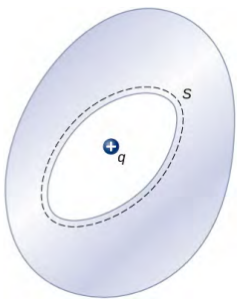
\includegraphics[width=0.35\textwidth]{figures/jittFigure1.png}
\caption{\label{fig:jittFigure1} From conceptual question 18 in the text.}
\end{figure}
\end{frame}

\begin{frame}{JITT 1.6}
\small
``The conductor will experience  an electrical field from q.'' \\
``yes it will it will experience the a charge of the same as the charge inside the cavity, either positive or negative'' \\
``yes, gaussian radius is greater than conductor's radius. '' \\
``yes because the q will be positive inside the cavity'' \\
\end{frame}

\section{Gauss's Law}

\begin{frame}{Gauss's Law}
Let $\vec{A}$ be a vector that:
\begin{itemize}
\item has a magnitude equal to the area of a surface
\item has a direction that is orthogonal to the surface
\end{itemize}
If a surface has area $A$, then $\vec{A} = A \hat{n}$, where $\hat{n}$ is normal, and pointed outward orthogonally from the surface.  What does \textit{outward} mean?
\end{frame}

\begin{frame}{Gauss's Law}
\begin{figure}
\centering
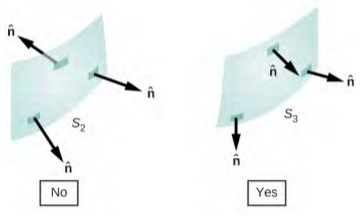
\includegraphics[width=0.5\textwidth]{figures/areaVector.png}
\caption{\label{fig:n} The convention for the area vector direction is outward, not inward.}
\end{figure}
\end{frame}

\begin{frame}{Gauss's Law}
\begin{figure}
\centering
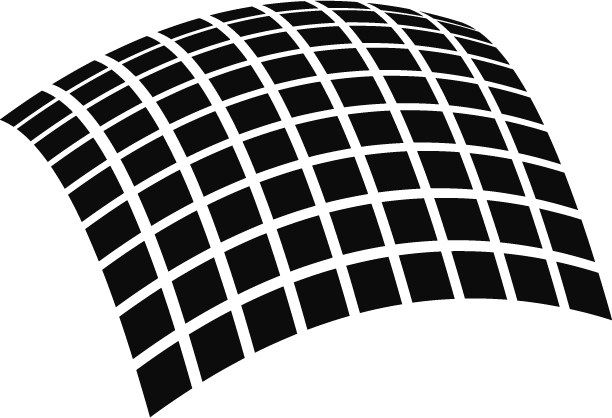
\includegraphics[width=0.5\textwidth]{figures/patch.png}
\caption{\label{fig:patch} We may think of a surface $S$ as the sum of many infinitesimal square patches $dS_i$, each with an area vector $\vec{dA}_i$ equal in magnitude but not direction.}
\end{figure}
\end{frame}

\begin{frame}{Gauss's Law}
A rectangular surface has length $a$, width $b$, and it is located in the x-y plane.  What is the area vector of the rectangular surface?
\begin{itemize}
\item A: $b^2 \hat{k}$
\item B: $a^2 \hat{i}$
\item C: $ab \hat{k}$
\item D: $ab \hat{j}$
\end{itemize}
\end{frame}

\begin{frame}{Gauss's Law}
\small
\begin{figure}
\centering
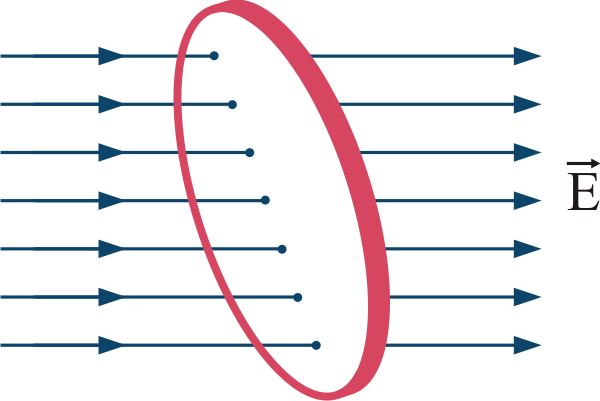
\includegraphics[width=0.5\textwidth]{figures/coin.png}
\caption{\label{fig:coin} A circular patch, with an external electric field.  How many electric field lines would pass through the circular patch if it was tilted to 90$^{\circ}$ from the field?  How about 0$^{\circ}$?}
\end{figure}
This behavior indicates a \textbf{dot-product} is working (zero and maximal over a span of 90 degrees).  But a dot-product of which two quantities?
\end{frame}

\begin{frame}{Gauss's Law}
Electric flux:
\begin{equation}
\boxed{
\Phi = \vec{E} \cdot \vec{A}} = E A \cos\theta
\end{equation}
Assumptions:
\begin{itemize}
\item $\theta$ is the angle between the area vector and the field
\item The electric field is uniform over this surface
\item The surface is flat
\end{itemize}
These assumptions do not hold for any arbitrary configuration of charge and surfaces.  However, if we zoom in closely enough to an individual patch, it does. \\ \vspace{0.5cm}
The units of electric flux are N C$^{-1}$ m$^2$.
\end{frame}

\begin{frame}{Gauss's Law}
How can we obtain the flux of more complex electric fields through more complex surfaces?  Simple: zoom in, get the flux from a patch, add it to the total:
\begin{equation}
\Phi = \sum_i^N \vec{E}_i \cdot d\vec{A}_i
\end{equation}
In situations like this, the summation usually becomes an integral if we make $dA$ small and $N$ very large.  That is, break the surface into many small patches.  But now we are dealing with two vectors, $\vec{E}$ and $d\vec{A}$...
\end{frame}

\begin{frame}{Gauss's Law}
\begin{equation}
\boxed{
\Phi = \int_{\rm S} \vec{E} \cdot d\vec{A}} \label{eq:flux}
\end{equation}
Equation \ref{eq:flux} is known as a \textit{surface integral.}  We can do these!  Let's try an easy one.  Let $\vec{E} = E_0 x \hat{k}$, and $S$ be a square of width $x_0$ and height $y_0$ in the x-y plane. \\ \vspace{0.5cm}
\textbf{Group board exercise:} Compute the electric flux $\Phi$, and check the units to make sure they are correct.
\end{frame}

\begin{frame}{Gauss's Law}
$\Phi = \frac{1}{2} E_0 y_0 x_0^2$.  (This has units of electric field times area).  Which of the following would increase the flux?
\begin{itemize}
\item A: If $x_0$ or $y_0$ were to grow larger
\item B: If $E_0$ were to grow larger
\item C: If $\vec{E}$ were directed at an angle to the z-axis
\item D: Both A and B
\end{itemize}
\end{frame}

\begin{frame}{Gauss's Law}
Imagine now that there is another, identical surface \textit{above} the first surface, but it is \textit{upside-down}.  The electric field passes through both surfaces.  What is the total flux, the sum of the fluxes through both surfaces?
\begin{itemize}
\item A: $\Phi = \frac{1}{2} E_0 y_0 x_0^2$
\item B: $\Phi = E_0 y_0 x_0^2$
\item C: $0$
\item D: $\Phi = -\frac{1}{2} E_0 y_0 x_0^2$
\end{itemize}
\end{frame}

\begin{frame}{Gauss's Law}
The answer is zero because, for the \textit{upside-down} surface, the area vector is in the direction $-\hat{k}$.  In fact, this result applies to any \textbf{closed surface}:
\begin{figure}
\centering
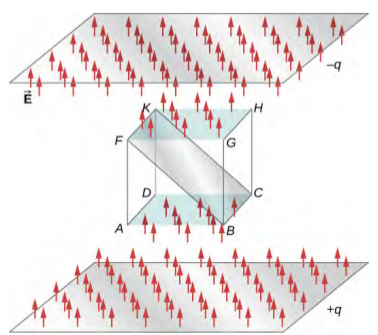
\includegraphics[width=0.4\textwidth]{figures/cube.png}
\caption{\label{fig:cube} The flux through a closed surface due to an external field is zero.}
\end{figure}
\end{frame}

\begin{frame}{Gauss's Law}
We can encapsulate this idea in the following equation:
\begin{equation}
\boxed{
\Phi = \oint_{\rm S} \vec{E}_{\rm ext} \cdot d\vec{A} = 0} \label{eq:ext}
\end{equation}
In general:
\begin{equation}
\boxed{
\Phi = \oint_{\rm S} \vec{E} \cdot d\vec{A}} \label{eq:general}
\end{equation}
However this implies something interesting about closed surfaces.  If the flux is non-zero through a closed surface, the field cannot be an external field.  It has to be an \textit{internal field}.
\end{frame}

\begin{frame}{Gauss's Law}
How do you make an electric field \textit{internal} to a closed surface?  How do you make an electric field in general?  \textbf{Charge.}  Charge is the origin of any electric field.
\begin{equation}
\boxed{
\Phi = \oint_{\rm S} \vec{E} \cdot d\vec{A} \propto Q} \label{eq:general2}
\end{equation}
If the charge $Q$ is outside the surface, then by definition the field is external to the surface.  If the surface \textit{encloses the charge}, then the total flux is non-zero, and\footnote{Formal proof relies on the \textit{divergence theorem}, from Calculus III.}
\begin{equation}
\boxed{
\frac{Q_{\rm enc}}{\epsilon_0} = \oint_{\rm S} \vec{E} \cdot d\vec{A}} \label{eq:gauss}
\end{equation}
\end{frame}

\begin{frame}{Gauss's Law}
A charge $Q$ is at the origin.  Compute the electric field via Gauss's Law, at $P = (0,0,R)$. \\ \vspace{0.5cm}
\textbf{Group board exercise.}
\end{frame}

\section{Conclusion}

\begin{frame}{Unit 3 Summary}
\textbf{Reading: Chapters 5-7}
\begin{enumerate}
\item Charge, Conductors and Insulators
\item Coulomb's Law and Electric Fields
\item E-fields of Charge Distributions
\item Gauss's Law
\end{enumerate}
\end{frame}

\section{Answers}

\begin{frame}{Answers}
\tiny
\begin{columns}[T]
\begin{column}{0.5\textwidth}
\begin{itemize}
\item It is zero.
\item Entropy has increased, but the internal energy returns to the original value
\item 0.5
\item The system does work equal to 0.5 liters times 1 atm
\item +1
\item The negative charges in the conductor move toward the positive charges in the rod.
\item The charges accelerate towards each other.
\item The charges $-2q$ accelerate towards the charge $+q$.
\item They are probably $\vec{v}_{\rm i} = -\hat{i}-\hat{j}$
\item They are probably $\vec{v}_{\rm i} = \hat{i}-\hat{j}$
\item 45 deg
\item Symmetry
\item About 25 deg (26.56 degrees)
\item Taking the value $z = R$ represents a minimum in the field strength.
\item The field is constant.
\item $\frac{\sigma}{\epsilon_0}$ N/C
\item 0 N/C
\end{itemize}
\end{column}
\begin{column}{0.5\textwidth}
\begin{itemize}
\item The total charge on the ring
\item A point charge $Q_{\rm tot}$
\item $ab \hat{k}$
\item Both A and B
\item $0$
\end{itemize}
\end{column}
\end{columns}
\end{frame}

\end{document}
